\documentclass[]{report}
\usepackage[english]{babel}

\usepackage{url}
\usepackage{cite}
\usepackage{graphicx}
\bibliographystyle{apalike}
\pagenumbering{roman}

\setlength{\parindent}{0pt}
\setlength{\parskip}{5pt plus 2pt minus 1pt}

% Title Page
\title{Augmented Reality mirror game}
\author{Thijs Boumans \and Patrick Kramer \and
        Alexander Overvoorde \and Tim van Rossum}
\begin{document}
\maketitle

\begin{abstract}
This report describes the procedure of development of an augmented reality game
for the TU Delft. This game, called the \emph{Augmented Reality Mirror Game},
is a game that uses augmented reality technology to simulate lasers, mirrors,
a target (or multiple targets), and walls. The goal of this game is to use
mirrors to deflect the laser beam coming from the laser to the target.
%TODO: add description of the chapters.
\end{abstract}
\tableofcontents
\listoffigures
\chapter*{Summary}
	Augmented reality can be best described as viewing a real-world environment
	which contains elements that have been generated by a computer. Basically,
	a real-world view containing computer-rendered elements. There are multiple
	hardware components to make an augmented reality view of the world possible,
	as well as multiple programs to use a real-world view, insert several
	elements and create an augmented reality environment.

\chapter{Orientation} \label{cha:orientation}
\pagenumbering{arabic}
	This chapter provides an overview of the orientation phase of the project.
	It shows an analysis of the project requirements, and the decisions that
	have been made during the project regarding choices of frameworks and
	libraries as well as game play elements. It also functions as a thorough
	introduction to this report.

	For a more in-depth view on the research that has been done leading to
	these decisions, please refer to the Research Report in appendix
	\ref{app:researchreport}.

	\section{Project Description} \label{sec:projectdescription}
		While augmented reality research has grown into a mature field over the
		last years, the aspects of situational awareness and presence of
		augmented reality (AR) are still quite open research topics. This
		project is about designing and implementing a collaborative game to
		explore the different perception of situational awareness, presence and
		workload in a physical and an AR environment. The game is to be employed
		as an approximation of collaboratively solving complex problems, as they
		occur in crime scene investigation when using virtual co-location, i.e.
		expert remote crime scene experts to guide local investigators in
		AR to collaboratively analyze the crime scene.

	\section{Final Product} \label{sec:finalproduct}
		The goal of the game is to solve a puzzle by controlling laser beams
		using mirrors in such a way that a predefined target is hit. The game
		can be played by one or more local players and one or more remote players.
		
		There are cards present for the local players that represent mirror
		bases. These must be placed on the table, which will be the locations
		for the mirrors. The local players will be able to see the mirrors they
		place through the use of AR technology. Each of the local players will
		only be given a few of the mirror bases needed to solve the puzzle, and
		as such solving it requires cooperation from all local players.
		
		The remote players can also see the placed mirrors, and can rotate them
		to influence the path of the laser beam(s). Only by cooperation between
		local players (who can only move the mirror bases) and remote players
		(who can only rotate them) it becomes possible to hit the target and as
		such solve the puzzle.
		
		The game provides various types of objects with different capabilities, 
		allowing for more complex puzzles. Examples of such objects include,
		but are not limited to walls, laser beam splitters and checkpoints.
		For a complete overview of the game objects provided by the game, see
		section \ref{sec:graphicaldesign}.
		
		The game is designed to stimulate cooperation between physically
		co-located players and the remote player(s). It does so by
		dividing abilities required for solving the puzzles amongst all players
		as follows:
		
		\begin{itemize}
			\item Physically co-located players each get only a part of the
			mirror bases required to solve the puzzle, requiring input
			from all of these players.
			\item If there are multiple physically remote players, each of
			these can only rotate a subset of the mirrors, and
			as such input from all physically remote players is
			required for solving the puzzle.
			\item Physically remote players have the ability to rotate
			mirrors while the physically co-located players do not have
			this ability, requiring input from both physically co-located
			as well as remote players.
		\end{itemize}
	
	\section{Software Design Methods} \label{sec:designmethods}
		This section describes the design methods that were used during the
		project. It illustrates the methodology that wasere d to develop and
		coordinate the project during the development phase.
	
		\subsection{Design Process} \label{ssec:designprocess}
			In designing and implementing the product, it is important that
			requirements can be changed quickly and without much problems. This is
			not because the requirements are likely to change from the client
			side, but because the choice of AR technology may change over the
			course of the project because of technical issues. The available Virtual
			and Augmented Reality glasses are mostly still in development, and as
			such this may affect the technical viability of each device.
			
			To deal with such changes, we use the Scrum methodology. This
			methodology describes a set of rules that, amongst others, makes it
			easier to deal with various changes during the development process.
			For a complete description of the rules that the Scrum methodology
			describes, please refer to the Scrum guide, available at
			\url{http://www.scrumguides.org/scrum-guide.html}. The methodology
			in graph form can be seen in \ref{fig:scrum}. The methodology
			shown is nearly identical to what we use, the only 
			exception being that our sprints only last one week instead of two.
			
			\begin{figure}
			\centering
			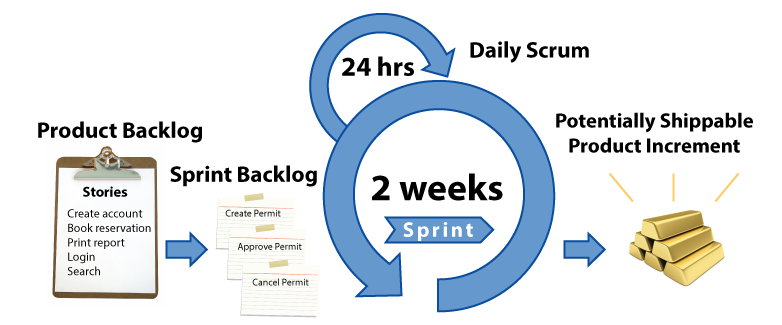
\includegraphics[width=\textwidth]{Scrum}
			\caption{Scrum methodology overview}
			\label{fig:scrum}
			\end{figure}
		
		\subsection{Organization} \label{ssec:organization}
			To be able to simultaneously work on the project without conflicts, we
			use Git as a version control system. The project is stored remotely on
			GitHub, ensuring the work is efficiently shared between all team members.
			Also, Git stores all commits that have been done. These can be reviewed
			on GitHub, and it is possible to go back to a commit stage if we
			absolutely need to, in case of something horribly wrong happening to
			the project.
			
			To coordinate and divide the tasks, as well as to maintain the items in
			the Scrum backlog, we use Trello. Trello is an on-line service that
			provides a dynamic way to organize items in various lists. It does
			so by using cards as bullet points in a list. It is also possible to
			assign certain people to those cards, which can be used to visibly
			divide tasks among the group members. Using labels, each card can also
			be categorized as a task relating to a certain part or parts of the
			project, such as software engineering, graphics design, networking,
			etc. We created lists to keep track of which items were in the backlog, 
			which items were being worked on and which items were already done.
			This allowed us to easily see what was being done and what was done.
			
			The project is licensed under the terms of the MIT license. We chose
			this license because it allows other developers to learn from this
			project. Additionally, since this project is done as a part of a
			research project, we believe making it open source may
			help future researchers in the same field. The full terms of the MIT
			license can be found at \url{http://opensource.org/licenses/mit-license.html}
			
			%TODO Move this paragraph to correct sections in the Quality Assurance chapter.
			To ensure the C\# source code in the project meets common coding standards
			(as set by Microsoft), we use the code analysis tools FxCop and StyleCop
			in combination with SonarQube. FxCop performs static code analysis, like
			code complexity and some naming conventions. StyleCop, on the other hand,
			focuses more on code style which includes use of spacing and
			documentation as well as other factors. SonarQube is a platform that
			unifies the reports from these tools and provides a clean overview of the
			combined issues found by FxCop and StyleCop, as well as some simple metrics
			SonarQube has built-in.
			
		\subsection{Design Architecture} \label{ssec:designarchitecture}
			Because the product is a game and the goal of the project is more
			focused on the game mechanics rather than the underlying engine, we chose
			to use Unity as a starting point. Unity provides a platform independent
			development environment for creating games, and offers many features 
			commonly used in games.
			
			Using Unity means that the project architecture is bound to the
			loosely coupled component-based architecture that Unity provides,
			although it is possible to include principles from object-oriented
			programming to some extent.
			
		\section{Process}\label{sec:process}
			This section describes the process of the project. The different phases
			during the project are highlighted in this section.
		
		\subsection{Early Preparations} \label{ssec:preparations}
			Before the project started, we had a meeting halfway through March
			with our coach about what the project entails and what is currently
			possible, given the hardware that we have today. After a brainstorm
			session and a pitch session with our coach and client, we were shown 
			what kind of hardware the TU Delft has available, and also what the 
			limitations of this hardware are. In this phase, a product plan was
			also created. This document describes the planning for the duration
			of the project, and can be found in appendix \ref{app:productplan}.
		
		\subsection{Research} \label{ssec:research}
			The first two weeks were the main research phase. This entailed that the
			research report had to be written. The second week was partly devoted
			to writing the report, and also to testing out more functionality of
			the software and hardware. The first game object models were also
			developed during this time, and there were plans for a first demo at the end
			of week 3 or at the beginning of week 4. The research report, which was the 
			result of these two weeks, can be found in appendix \ref{app:researchreport}
		
		\subsection{Programming the basic game} \label{ssec:basics}
			The next two weeks revolved around creating game objects and game play.
			After some testing with markers and AR glasses, as well game objects, a 
			first demo was also developed during this time. This phase also saw unit testing of g
			elements, as well as heavy usage of StyleCop and SonarQube to clean up
			respectively reorganized code in order to deliver clean code to SIG, for our first
			submission.  
		
		\subsection{The OpenCV server} \label{ssec:firstdemo}
			Week 5 finally saw the first demo being demonstrated to the coach. The
			coach was satisfied, but there was a lot to be done before the project
			could be considered finished. During this week, networking was revamped
			and development of a server that makes use of the computer vision library
			OpenCV started. This decision was based on various technical challenges we 
			came across during development. The reason for this decision can be found 
			in the Implementation chapter (chapter \ref{cha:implementation}).
		
		\subsection{Restructuring the entire project}
			Week 6 began with a massive restructuring of the project. Right before
			the code was to be handed in to SIG, Unity failed to build the project
			completely. There were no errors in the scripts, but the Unity compiler
			kept throwing unexplainable error messages. This caused us to move 
			everything that we wanted to move from the original project to a new
			Unity project.
			
			Even though this caused a setback in the project planning, this issue
			gave us an opportunity to take a critical look at our code base. After
			completing this task and handing in the package for SIG, development 
			could continue on the OpenCV server. The results for the SIG evaluation
			from this week can be found in appendix \ref{app:sig1}.
		
		\subsection{The new projection code}
			Week 7 began with further development on the OpenCV server and the code
			needed for correct projection of the META One. The projection code base
			was overhauled on Monday, mainly to allow for better unit testing. During
			this week, the midterm meeting also took place, and we could show off
			what we had up until that point. The coach and the customer(s) (Stephan
			could not be there, so he sent some of his colleagues to check in on
			how the project went) were impressed, but they also said that development
			had to continue for the time being. At the end of week 7, the server was
			completed, but now the true challenge began: integrating all the software
			into one single product.
			
			Week 8 started with the integration of all the parts of the software.
			From the start on, this proved quite challenging. Players could rotate
			mirrors by rotating the markers (which shouldn't happen, as this would
			kill off the co-operative element of the game), as well as other things.
			As such, development on projection code was once again necessary.
			Throughout this week, massive progress was made towards integration of 
			the various parts of the software, especially from early Wednesday on.
			Because of the progress considering integration of software, level design
			could finally start.
		 
		\subsection{Further integration}
			Week 9 was even further devoted to integration of all the various bits and
			pieces of the software. Once again, massive progress was made in
			integrating all software, and at the end of the week, the first fully
			working version was finally released. 
		 
		\subsection{Wrapping up}
			At the end of week 10, the final report had to be handed in. This meant
			that the project had to be wrapped up.
		 
		\subsection{The process table} \label{ssec:processtable}
			The following table gives a nice and short overview regarding what was done
			every week. An X in a particular subproject and week means that, during that
			week, that subproject was developed further.
			
			\begin{table}[!ht]                                                                                      
				\begin{tabular}{| c | c | c | c | c | c | c | c | c | c | c |}
				\hline
				Weeks             & 1      & 2      & 3      & 4      & 5      & 6      & 7      & 8      & 9      & 10     \\ \hline
				Research          & X      & X      & \space & \space & \space & \space & \space & \space & \space & \space \\ \hline
				Final report      & \space & \space & \space & X     & X      & X      & X      & X      & X      & \space \\ \hline
				Networking        & X      & X      & \space & \space & X      & X      & X      & \space & X      & \space \\ \hline
				Augmented reality & \space & \space & \space & X      & X      & X      & X      & X      & \space & \space \\ \hline
				Game elements     & X      & X      & X      & X      & \space & \space & \space & \space & \space & \space \\ \hline
				Testing           & \space & \space & X      & X      & X      & X      & X      & X      & \space & \space \\ \hline
				Projection        & \space & \space & \space & X      & X      & X      & X      & X      & X      & \space \\ \hline
				Level design      & \space & \space & \space & \space & \space & \space & \space & X      & X      & \space \\ \hline
				\end{tabular}
			\end{table}

\chapter{Design} \label{cha:design}
	This chapter explains the design of the system. This includes: back-end
	design, model/graphical design, and main activities.

	\section{Main activities} \label{sec:mainactivities}
		There are several main activities in the system, corresponding to the two
		main user types of the system. These user types are both the physically co-
		located	players as well as the physically remote players. The activities
		are as follows:

		\subsection{A local user wants to start a game} \label{ssec:userstartgame}
			The local user ensures the main camera is set up according to the 
			provided guidelines. The local user then starts the server on the 
			machine the camera is connected to. The local user needs to take note 
			of the IP address of the server machine and fill this into his local 
			machine (to which the Meta One glasses are attached). The other players
			also fill in the same IP address. The server can also run on one of the 
			players' machines. The local user needs to wait for others to join the 
			game. When at least two local players and at least one remote player 
			has joined the game, the game will start.
			
		\subsection{A local user wants to join a game} \label{ssec:localjoingame}
			A local player wants to join an active game. Before this can
			happen, a game has to be started first. The local player needs to 
			acquire the IP address of the server machine and fill this in.
			Once the game starts, the local player will see virtual objects projected 
			through the Meta One glasses.

		\subsection{A remote user wants to join a game} \label{ssec:remotejoingame}
			A physically remote player wants to join an active game. Before this can
			happen, a game has to be started first. The remote user needs to acquire 
			the IP address of the local server machine (see \ref{ssec:userstartgame})
			and fill this in. The remote user will see a virtualized version of the 
			same game world as the local players.

	\section{Back-end design} \label{sec:backenddesign}
		The system is composed of three main parts: The Laser mechanics, the network
		functionality and the projection to 3D glasses. For this purpose, we divided
		the C\# code over three namespaces, named "Core", "Network" and
		"Projection", respectively.

		The "Core" namespace is responsible for drawing the Laser beams and
		providing the interactions of laser beams with the other game objects.
		The layout of this namespace is discussed in paragraph 
		\ref{ssec:corenamespace}.

		The "Network" namespace is responsible for synchronizing the game state
		between all connected players. The layout of this namespace if discussed 
		in paragraph \ref{ssec:networknamespace}.

		The "Projection" namespace is responsible for providing the projection to
		the VR glasses. This namespace provides the functionality required to project
		the game world to the VR glasses. The layout of this namespace is discusses in
		paragraph \ref{ssec:projectionnamespace}.
		
		Additionally, the game depends on the deployment of a server application written
		in C++. The purpose of this server application will be discussed in
		\ref{ssec:networknamespace}.
		
		\subsection{The Core namespace} \label{ssec:corenamespace}
			%TODO: Write about core namespace.
			
		\subsection{The Network namespace} \label{ssec:networknamespace}
			%TODO: Write about network namespace.
					
		\subsection{The Projection namespace} \label{ssec:projectionnamespace}
			%TODO: Write about projection namespace.

	\section{Game elements} \label{sec:graphicaldesign}
		For designing the 3D models, we used Blender. Blender is a free application
		for 3D modeling, under the GPL license, and Unity natively support Blender models (provided Blender is installed on the system). We have chosen for a light looking style featuring nature inspired modeling and gold and crystal based materials. The light modeling style causes slight miss alignments with the ground to be less noticeable and makes the lack of feedback from moving a card feel less odd. The crystals and gold 
		just feels good in combination with the beams of light.
		The following sections display and describe the graphics used in
		the gameplay elements, as well as the function of
		these elements.
		% TODO Explain why we chose this graphics style
		
		\subsection{Laser target} \label{ssec:lasertarget}
			The laser target is the main target of the game. It consists of
			a small container, which contains a crystal. The point of the
			game is to direct a laser beam from an emitter to this target.
			When the target is hit by a laser beam, the outer columns around
			the crystal inside will rotate and spread out, indicating that
			the target has been hit. The game will then proceed to the
			next level. An image of the target is shown in figure 
			\ref{fig:target}.
			\begin{figure}[h]
				\centering
				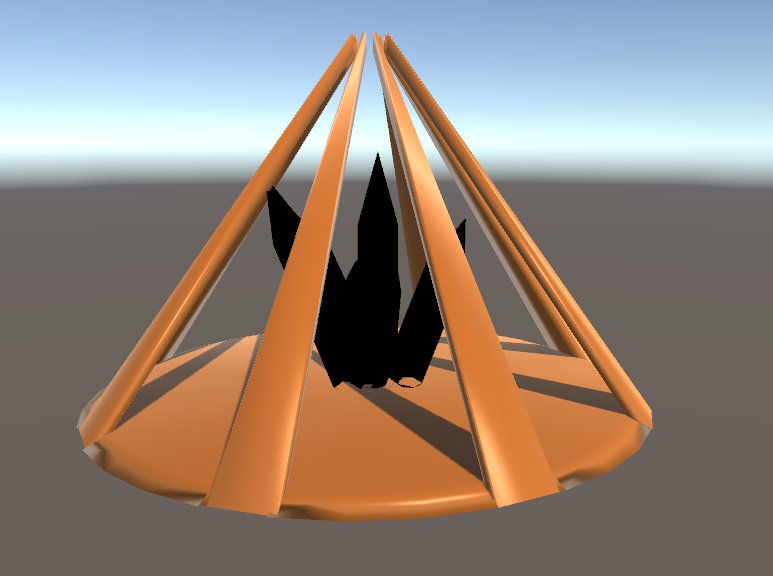
\includegraphics[width=\textwidth]{Target}
				\caption{the target of the game. The gold columns around the inner crystal will open up and rotate once the target is hit, as described earlier. Also, the crystal will change color once the target hits it.}
				\label{fig:target}
			\end{figure}
			
		\subsection{Mirror} \label{ssec:mirror}
			A mirror is a crucial game element. Its reflective surfaces
			allow it to reflect any laser beam that hits these surfaces.
			It is also the only element that players can move and/or rotate.
			All levels require at least one mirror to move or rotate
			in order to hit the target. An image of a mirror in-game is shown
			in \ref{fig:mirror}.
			\begin{figure}[h]
				\centering
				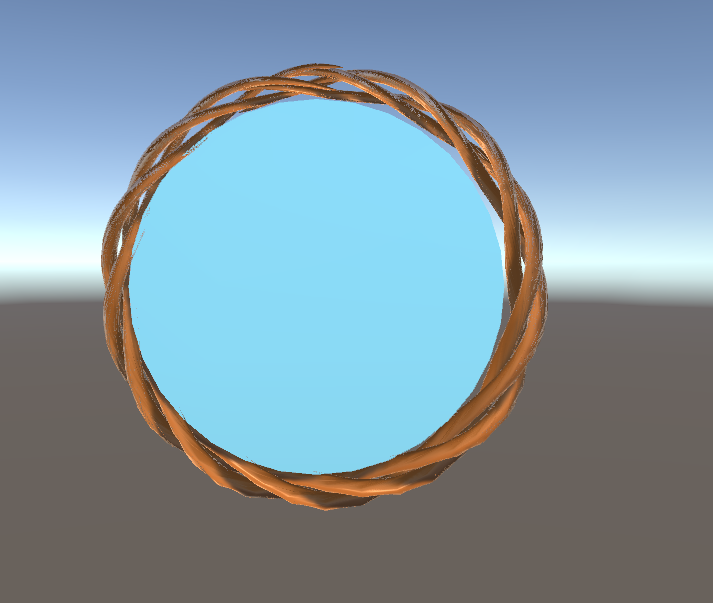
\includegraphics[width=\textwidth]{Mirror}
				\caption{an image of a mirror in-game, with its reflective surfaces.
				The light blue circles reflect laser beams, the golden outer frame
				does not.}
				\label{fig:mirror}
			\end{figure}
			
		\subsection{Wall} \label{ssec:wall}
			The wall is the main obstacle in the game. It blocks incoming
			laser beams completely. Walls are used in levels to make it 
			less easy for one player to reflect a laser beam coming from
			an emitter to the target. The first few levels mainly use walls
			to create paths that the laser beam has to go through, later
			levels use not only walls, but also other game objects.
			
		\subsection{Emitter} \label{ssec:emitter}
			The emitter is the most important aspect of the entire game.
			It is the only "true" source of a laser beam (although game
			elements like the beam splitter can also create beams, these
			elements always require input in the form of another laser
			beam; the emitter does not have that problem, hence it is a "true"
			source). In the early levels, players only move and rotate mirrors
			to guide a laser beam from the emitter to the target, while in the
			later levels beams have to be guided towards other game elements
			(like the beam splitter, for example) in order to complete the
			level. It is possible to have multiple emitters in a single level,
			and later levels use this to create more complex puzzles.
			What the emitter looks like exactly is shown in figure 
			\ref{fig:emitter}.
			\begin{figure}[h]
				\centering
				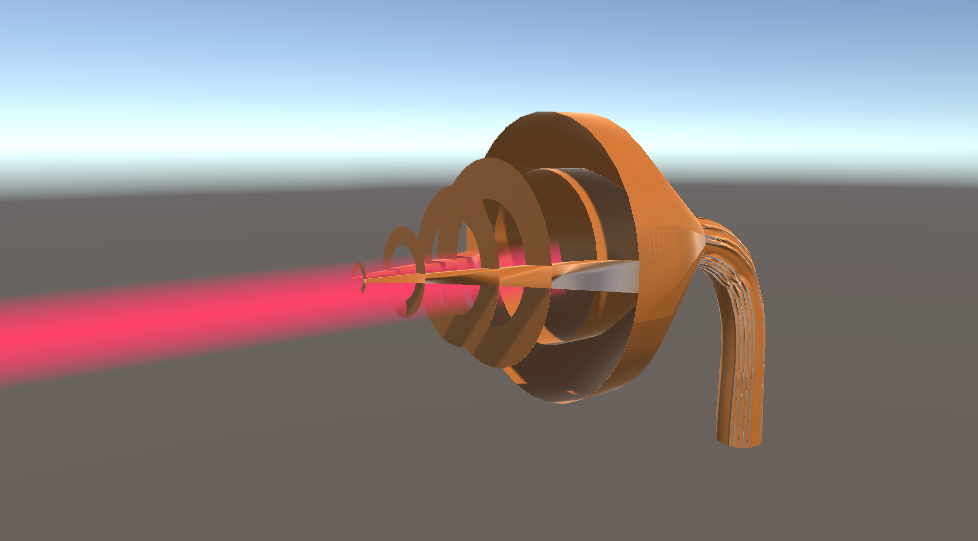
\includegraphics[width=\textwidth]{Emitter}
				\caption{what the emitter looks like in the game. Also shown here is a laser beam
				coming from the emitter. The laser beam is colored red per standard. There are game objects that can change the coloring of the beam, these will also be described in this part of the report.}
				\label{fig:emitter}
			\end{figure}
\chapter{Implementation} \label{cha:implementation}
    The Bachelor Project course would not be a real Bachelor Project course if 
    there were projects without technical challenges whatsoever regarding the 
    implementation of the final result. Therefore, this chapter elaborates
    on the technical challenges faced during development of the project and
    the solutions that we have developed for these challenges.
    %TODO Highlight technical challenges and elaborate on solutions for these challenges.
    %     This includes (amongst others) how the AR functionality posed a problem and we
    %     implemented a C++ server using OpenCV to take over that work (along with 
    %     synchronizing on a central camera).
    
    % Sections are purely by example. This list might not be entirely correct or complete.
    \section{AR Glasses} \label{sec:arglasses}
        One of the first design choices that we had to make was about what
        AR glass was going to be used with the project. As can be seen in
        our research report, under appendix \ref{app:researchreport},
        there two options to choose from. These were the Oculus and
        the META One. We eventually settled for the META One, because
        of the latency of the Oculus. A pair of META Glasses can be seen in
        figure \ref{fig:metaone}.
        
        \begin{figure}[!ht]
            \centering
            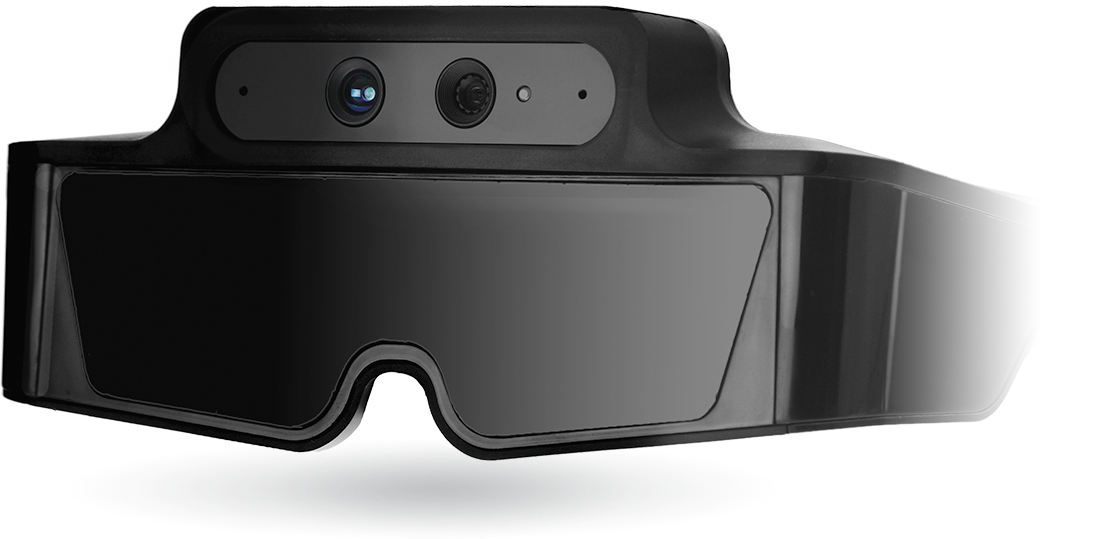
\includegraphics[width=\textwidth]{MetaOneGlasses}
            \caption{A pair of META One glasses.}
            \label{fig:metaone}
        \end{figure}
        
        The challenge with the META One was to get it working in Unity.
        There is a Meta SDK which allows for Unity games to work with
        the META One, but AR itself is still in development (as of
        writing this report), and the META One glasses are experimental
        at best. The SDK that we used first was also very buggy (due to the
        experimental nature of the META One). Also, the META One has a very
        limited field-of-view (the field-of-view was so limited that, during
        one of our first tests with our coach, the coach had to sit back
        to keep everything tracked, which, especially considering that they
        had to move markers as well as track the environment continuously,
        was less than ideal). However, the SLAM tracking built into the
        META allows for game objects to continue to be rendered on a marker
        even if the marker is outside of the view of the META. SLAM tracking
        is explained in subsection \ref{ssec:slamloc}.
        
        \subsection{SLAM tracking} \label{ssec:slamloc}
            SLAM is an acronym, which means Simultaneous Localization And
            Mapping. It stands for a computational problem making a map
            from an unknown environment while updating the location of the
            agent in the same environment. These problems cannot be solved
            independently from each other, as updating a map usually involves
            knowing the location of the agent before any accurate updates
            can be made, and vice versa. Several algorithms have been developed
            for solving this problem, and there is even a platform, called OpenSLAM,
            which contains several open source algorithms which solve this
            problem.
            
            However, the algorithms are beside the point. the real benefit of 
            using SLAM with AR is that SLAM tracking allows the META One to
            render the game objects belonging to a marker while keeping them
            rendered once the marker leaves the field-of-view of the META One.
            Considering that the field-of-view of the META One is not that large
            (As seen in our research report under Appendix \ref{app:researchreport}),
            this is a huge benefit. The META One also has built-in support for
            SLAM tracking of objects, which meant that no time had to be spent
            on developing algorithms.


    \section{Synchronization of World State} \label{sec:synchronization}
        Because the game is played by multiple people, the state of the world
        somehow has to be synchronized between all players. To do this, we 
        considered two major options:
        
        The first option was to use the built-in Network View component in 
        Unity. This would allow Unity to take care of most synchronization,
        which in turn could make implementing the synchronization particularly
        easy. However, due to the way the Meta One glasses manipulate the 
        positions and rotations of game objects to fit the orientation of the 
        player's head, synchronizing these positions would result in incorrect
        positions for other players. Instead, a custom serialization method 
        would have to be implemented to undo the manipulation by the Meta One
        and then apply the correct manipulation for each of the other players.

        Another option was to introduce a master server with camera that hosts
        the game, and provides raw positions and rotations of markers exactly as
        they were placed on the table. The only thing left to do would be to
        move and rotate the objects for each player to match that player's view
        of the playing area.

        We chose the second option for the following reasons:

        \begin{itemize}
            \item A master camera can see all markers at any one time, which
            means that there is never any uncertainty.
            \item The first option requires complex peer-to-peer synchronization
            and conflict resolution when multiple players see an overlapping set
            of markers.
            \item Unlike the cameras worn by players, the master camera is not
            constantly moving, meaning that marker recognition is not affected
            by motion blur.
        \end{itemize}
        
        Aside from the aforementioned reasons, we also made the decision to go
        with the second approach because it allowed us more control over the 
        internal workings of the network functionality and the marker tracking.
        See section \ref{sec:markerdetection} for the details about the marker
        detection performed by the server.

    \section{Marker Detection} \label{sec:markerdetection}
        The META One glasses come with marker detection built-in and we had
        difficulty replacing this detection with a custom system. That meant
        that our master camera server has to detect the same type of marker.
        Luckily the META markers have a very simple design. They're 6 by 6 bits
        encoded as black and white squares with a black border around them, as
        shown in figure \ref{fig:metaonemarker}.

        \begin{figure}[!ht]
            \centering
            
\includegraphics{MetaMarker}
            \caption{A marker that can be recognized by the Meta.}
            \label{fig:metaonemarker}
        \end{figure}

        These patterns map to an ID and are asymmetrical so that rotation can be
        resolved when they are detected. To easily find these markers on a table
        and board, we've also added a vibrant green border to them. This doesn't
        affect the META, but it makes segmentation of the markers from the
        background much more straightforward for the master camera. These final
        markers are shown in figure \ref{fig:finalmarker}.

        \begin{figure}[!ht]
            \centering
            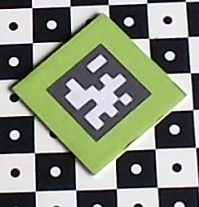
\includegraphics{FinalMarker}
            \caption{A marker that can be recognized by the Meta and the master camera.}
            \label{fig:finalmarker}
        \end{figure}

        The corners of the playing surface were originally set using red
        markers, as shown in figure \ref{fig:cornermarkers}. The need for these
        corner markers is explained in the next sections, which also describe
        the rest of the marker tracking process on the server.

        \begin{figure}[!ht]
            \centering
            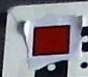
\includegraphics{CornerMarker}
            \caption{Original marker that indicates a playing surface corner.}
            \label{fig:cornermarkers}
        \end{figure}

        \begin{figure}[!ht]
            \centering
            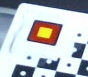
\includegraphics{CornerMarker2}
            \caption{New marker that indicates a playing surface corner.}
            \label{fig:cornermarkers2}
        \end{figure}

        \subsection{Board detection}
            The first step to tracking is to isolate the playing surface from
            the camera image and to apply perspective correction to it. The red
            corner markers described above are used to find the bounds of the
            rectangular playing surface. An example of the transformation is
            shown in \ref{fig:boarddetection}.

            \begin{figure}[!ht]
                \centering
                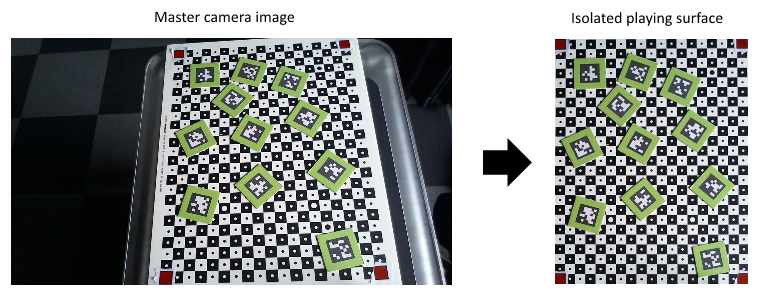
\includegraphics[width=\textwidth]{BoardDetection}
                \caption{Example of detecting playing surface and isolating it.}
                \label{fig:boarddetection}
            \end{figure}

            The four red corner markers are located by converting the input
            image to the HSV color space and thresholding on a red-like hue and
            a high saturation. The noise is then removed using a morphological
            open operation and the system verifies that 4 contours are found. If
            an amount of contours other than 4 is found, the user is prompted to
            move the camera such that the entire playing surface is visible and
            there are no other vibrant red objects in view.

            The corners of the playing surface are required to compute the
            transformation for the perspective correction. The perspective
            correction is required to recognize markers and their location
            correctly by making the camera view look like it views the board
            from above.

            We had some issues with these solid red markers. For example, a red
            chair near the testing setup was often also recognized as a corner
            marker. For that reason we designed a slightly more complex corner
            marker that has a yellow center, as depicted in figure
            \ref{fig:cornermarkers2}. Detection of this marker is the same as
            above along with a check for the yellow hole.

        \subsection{Marker detection}
            The markers are first segmented from the playing surface using their
            vibrant green borders, again through the HSV color space. The mask
            that results from this is cleaned up again using morphological open
            and close operations. An example of such a mask is shown in
            figure \ref{fig:markerthresholding}.

            \begin{figure}[!ht]
                \centering
                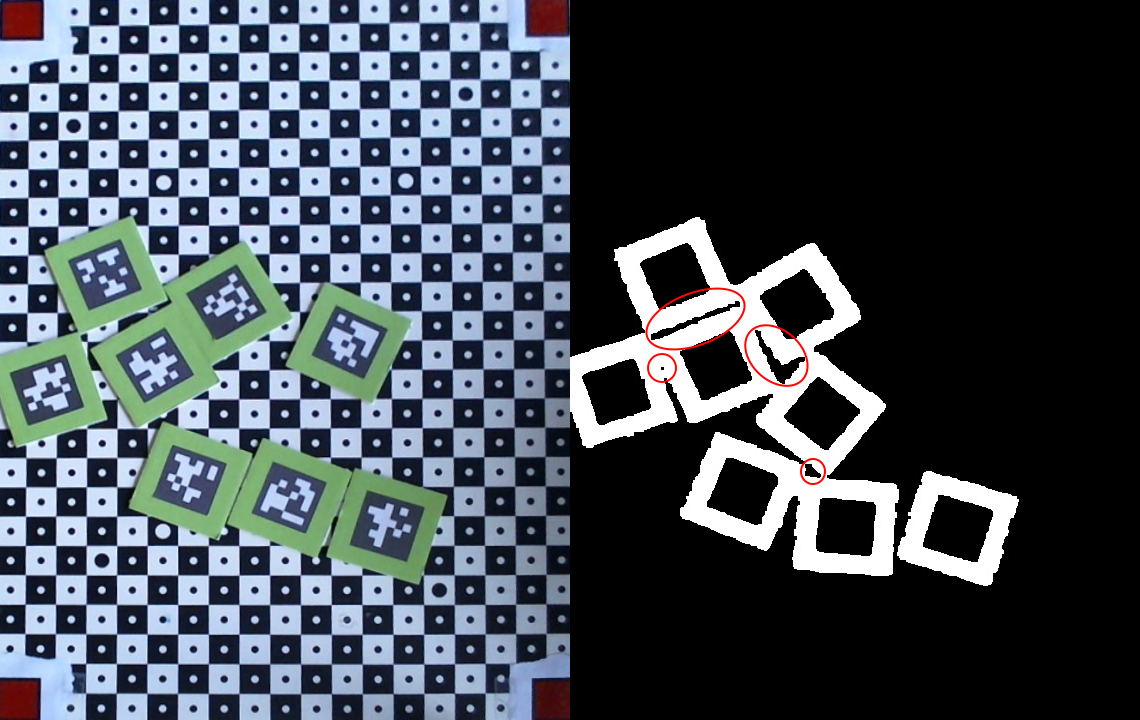
\includegraphics[width=\textwidth]{MarkerThresholding}
                \caption{Example of thresholding markers with false holes highlighted.}
                \label{fig:markerthresholding}
            \end{figure}

            It is evident from the example that finding the borders alone is not
            sufficient, because they will connect when the markers are close
            together. However, we know that each marker contains a non-green
            center with the actual code, which shows up as holes in the mask. We
            can detect these holes by using OpenCV's contour finding feature
            using hierarchy mode and selecting just the contours that lie
            directly within the outer contours.

            Unfortunately, when markers are really close together, some other
            holes appear as well (highlighted in the example). We remove these
            by filtering the contours using the following criteria:

            \begin{itemize}
                \item Holes have a minimum width and height of 8 (minimum
                required for reading a pattern)
                \item Holes are square to within a tolerance of 15\%
                \item Holes have the same size as the median size of all
                detected holes to within a tolerance of 15\%
            \end{itemize}

            Especially the last one works very well for a playing surface with
            many markers, where the signal to noise ratio is high. The process
            finished by returning the contours of all the holes detected as
            markers.

        \subsection{Marker recognition}
            The marker recognition process takes the contours from the marker
            detector stage. It starts by finding the minimum area bounding
            rectangle around a contour to find its rotation. The source image is
            then rotated to straighten the marker.

            The next step is to isolate the pattern from the marker. It first
            converts the image to grayscale and resizes it to 8 by 8 pixels (the
            6 by 6 pattern with the 1 pixel wide border within the marker). The
            average brightness across the pattern is found and used to threshold
            the black and white pixels. The image is then cropped to just the 6
            by 6 pixel pattern. The original scale of the marker is also stored
            to later scale the marker positions.

            The final step is to identify which known pattern the detected
            pattern best matches. Although the marker has already been
            straightened, it could still be rotated by 90, 180 or 270 degrees.
            For that reason, the system searches all known patterns using the
            four possible rotations of the input. It determines the best match
            using the Hamming distance between 2 patterns. The detected best
            matching rotation is then added to the rotation needed to straighten
            it to compute the complete rotation.

            The marker recognition system does not verify if the best pattern
            match is good enough, it will happily return a best match with
            confidence score \verb#0.0#.

        \subsection{Marker tracking}
            The marker tracker system takes the output from the marker detection
            and recognition stages (position and match) from each frame and uses
            this data to track the movement of markers across frames. It
            primarily does this by checking which marker position from the
            previous frame each new marker position is closest to. It uses the
            pattern matching results only when a marker is not moving quickly.
            It uses results from multiple frames to smoothen positions and
            rotations using a moving average that is discarded when a marker
            has sudden changes. It also detects if a marker has been removed by
            measuring if it hasn't been seen for a long while.

            All of the changes it detects, like new markers, moved markers and
            removed markers are added to a list each frame and returned to the
            main application. The main application then broadcasts these changes
            over the server socket to the META One clients.
        
    \section{Networking and the OpenCV server} \label{sec:network}
        The game depends on a server application with a master camera. The 
        server application detects the position and rotation of markers in the 
        playing area. It does this through the use of a central so-called master 
        camera, that is position so that the entire playing area is visible from 
        the camera.
        
        The server application is written in C++ and is based on OpenCV and the 
        Qt framework. We decided to implement the server outside of Unity, since 
        Unity does much more than what we need of the server. The server only 
        acts as a way to track all markers even if they aren't seen by any of 
        the players, and to facilitate synchronizing state changes with all 
        players. For example, if a remote player rotates an object in the game, 
        the details about that rotation is sent to the server, which then 
        distributes it to all other players.
        
        A more detailed description about the communication between the Unity 
        clients and the server can be found in paragraph \ref{ssec:communication}.
        The use of the master camera to detect markers is described in paragraph
        \ref{ssec:mastercamera}.
                
        \subsection{Communication between C\# and C++} \label{ssec:communication}
            Communication between the Unity clients and the OpenCV server 
            happens through the use of sockets. For the Unity side, the Socket 
            facility built into the C\# runtime is used. For the OpenCV server, 
            the TCP Socket facility of the Qt Network module is used for 
            providing a server socket capable of handling multiple clients. 
            
            The protocol used for communication is kept very simple to reduce 
            network load and for simplicity. The protocol consists of a number
            tag indicating the message type followed by the actual message 
            content. To facilitate the features the game provides, the following
            message types are used:
            
            \begin{description}
                \item[Position Update] Sent by the server whenever it detects a 
                                       change in a marker position.
                \item[Position Delete] Sent by the server whenever a marker is
                                       removed from the playing field.
                \item[Rotation Update] Sent by remote players to indicate they 
                                       have rotated an object. This message is 
                                       forwarded to all connected clients by the
                                       server.
\item[Level Update] Sent by players as soon as they consider the level to be finished. The server broadcasts it to the other clients to change the server.                                       
                                       
                \item[Ping Message]    Sent by the server and clients to indicate 
                                       they are still connected and listening.
                                      
            \end{description}
        
        \subsection{The master camera} \label{ssec:mastercamera}
            The master camera uses the tracking system described in section
            \ref{sec:markerdetection}. This system outputs the positions of the
            markers in pixels and rotations relative to the camera. The
            positions are normalized such that the width and height of a marker
            pattern is 1 unit. The detected scale from the marker recognition
            module is used to do this and is averaged across all markers and a
            couple of frames to ensure stability.

            The normalized positions and relative rotations are sent to the META
            clients using the communication protocol discussed in the previous
            section. Once they arrive, they are transformed into the META
            coordinate system using a "level marker". A "level marker" is an
            arbitrary marker detected by both the master camera and META
            built-in tracking system. The client can then transform the relative
            position of the other markers compared to the level marker from the
            server coordinate system to the META coordinate system. The rotation
            of the markers is compensated using the META detected rotation and
            the rotation received from the server.
\chapter{Quality Assurance} \label{cha:qa}
	This chapter explains and describes various quality assurance techniques 
	that were used during the project, to allow us to deliver a product of 
	good quality (regarding both code quality and gameplay quality). It also
	talks a bit about Microsoft Visual Studio first, our IDE of choice for
	this project, considering that some QA tools are not available for
	MonoDevelop, the standard IDE packaged with Unity.
	
	\section{IDE used for programming} \label{sec:ide}
		The IDE used for programming was Microsoft Visual Studio. Unity has an IDE
		of its own available for programming in C\#, which is called MonoDevelop.
		However, the MonoDevelop IDE is really lacking in functionality. It has no
		support for the plugins that we use to check our code. Furthermore, the use
		of MonoDevelop enforces a code style that is incompatible with the style 
		guidelines used by StyleCop (see \ref{sec:codestyle}), 
	
	\section{Testing} \label{sec:testing}
		There are three main types of testing done during the project. These are
		unit testing, integration testing and user testing. Unity has no native
		support for running unit\slash integration tests that have been written,
		but there is a toolkit available for free on the Asset Store, called
		Unity Test Tools,  that does have this support. The extension is
		developed by the Unity team, and can be found on the Unity Asset Store: 
		\url{https://www.assetstore.unity3d.com/en/#!/content/13802}.
		Using this extension, a new menu bar item, called "Unity Test Tools"
		will appear in the main Unity editor. Clicking on this item creates a drop
		down menu with different options, the most important one being the unit test
		runner.
		
		\subsection{C\# Unit Tests} \label{ssec:csharpunittests)}
			Unit tests are written using the NUnit unit testing framework for 
			C\#. NUnit is a test framework which was ported from the Java test 
			framework JUnit, and was created to bring xUnit testing to all .NET 
			languages. Using this framework is also really easy, and a tutorial 
			on how to write unit tests using NUnit can be found using Google. 
			Using Unity Test Tools, all unit tests in the project are listed 
			once one clicks on the subitem "Unit Test Runner". The tests are 
			listed in a new window, and one can run all unit tests by clicking 
			on the "Run All" button at the top. The menu then shows what unit 
			tests have passed or failed, and clicking on a unit test shows what 
			went wrong. A unit testing overview can be seen in \ref{fig:unitytesttools}.
			The UnityTest testing class seen in the overview also displays
			the different statuses of tests in the NUnit framework (passing,
			failing, inconclusive, not executed, and culture specific).
			
			\begin{figure}[!ht]
				\centering
				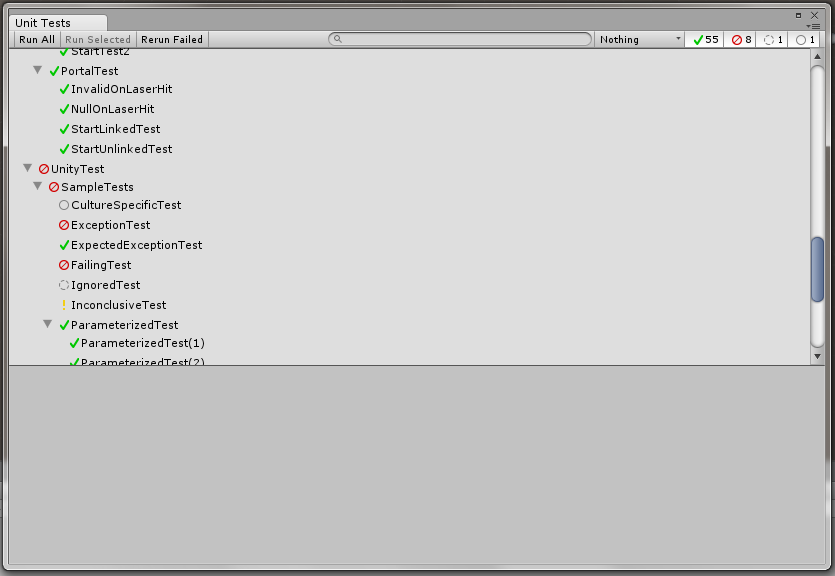
\includegraphics[width=\textwidth]{UnityTestTools}
				\caption{The Unity Test Tools unit testing screen.}
				\label{fig:unitytesttools}
			\end{figure}
			
		\subsection{C++ Unit Tests} \label{ssec:cplusplusunittests}
			The unit tests for the C++ server code are not written using the
			NUnit framework, as that would not really work. The framework for
			the tests in C++ is the Google Test framework. Google test is, like
			NUnit for C\# and JUnit for Java, an xUnit-based testing framework.
			As such, it also supports assertions, type parameterization, etc.
			Also, it is open source, licensed under the new BSD license.
			
            To implement the testing functionality into the server project, 
            the unit tests are separated into their own subproject, which 
            links to the server and runs the tests. As recommended by the 
            Google Test guide, the Google test framework source and headers 
            are included directly into the unit tests subproject, ensuring 
            that the tests can be compiled and run regardless of the platform 
            or compiler being used.
		
		\subsection{Integration Tests} \label{ssec:integrationtests}
			Integration tests are not done via a formalized test procedure, but 
			rather by creating simple scenes and observing that the subjects of 
			the test work as they should when they are placed in an actual 
			scene. It is also a lot harder to run these tests in a standardized 
			way most of the time.

		\subsection{User Tests}
			Although testing the code is important and it helps ensure that the
			software is working correctly, it doesn't tell us anything about the
			actual usability of the product. Since we're developing a game, it's
			especially important that the end users will have fun using the
			product. Properties like these can be evaluated by doing user tests.

			Most of the initial user testing will be done by us, the developers,
			because external parties will not have a good experience while it's
			still in the middle of development. This kind of user testing also
			comes automatically with developing the features of the game.

			In the last stage of development, when all of the technical
			challenges have been solved, we will be primarily working on the
			levels and gameplay of the game. It is no longer sufficient to just
			have the developers test the game by that point, because they will
			have an unrealistic playing experience. The developers will already
			be very familiar with the levels and game mechanics, which means
			that they won't be able to properly judge if the concepts are too
			hard to figure out for new players. By having a lot of other people
			playing the game, we'll be able to estimate if certain levels are
			too easy or too hard, and if all of the different game objects are
			fun to interact with. For example, if the beam splitter turns out to
			be too complex to use, we might remove it from the game.

			Finding other computer science students to play the game will not be
			a problem, but we will also try to find other demographics to test
			with. Computer science students are used to approaching logic
			problems like those in our puzzle game, which may give us a skewed
			idea of how hard the game is. If time allows for it, we could have
			high school students try the game as well in the Delft Science
			Center.
		
		\subsection{Code coverage} \label{ssec:codecoverage}
			Code coverage is a metric that can be used to determine how thorough
			the written code has been tested. We have to consider generating 
            code coverage reports for two languages: The C\# Unity project and 
            the C++ server project. 
            
            Generating code coverage reports for the C\# code is unexpectedly 
            difficuly: Even though here are several free software packages 
            available on the Internet that allow for generating code
			coverage reports of NUnit test suites, these are hard to use when 
            combined with unit tests in Unity. The reason behind this is that, 
            to run the unit tests for the game, the Unity Test Tools 
            functionality has to be used (as most tests use instantiation of 
            gameplay objects, something that canonly happen in Unity). This 
            functionality has no way of integrating the NCover or OpenCover 
            software packages. It is possible to integrate these with Microsoft 
            Visual Studio, however it is impossible to run the unit tests from 
            that IDE. As such, we had to manually check if the tests tested all 
            possible branches of the code.
            
            On the other hand, however, analysing code coverage for the C++ 
            project is almost trivial: For GNU compilers, including MinGW, 
            there is a utility called gcov, which measures code coverage of 
            GTest-based unit tests. And when using the Microsoft Visual C++ 
            compiler, it is possible to use Visual Studio to analyse the 
            coverage of the unit tests.
			
	\section{Code Style} \label{sec:codestyle}
		We decided to stick to the code style guidelines defined by StyleCop and 
		FxCop, two utilities developed by Microsoft. These utilities check for 
		common programming and code style errors in projects so that these can 
		easily be identified and fixed. 
		
		During the project, we kept the source code style checked by periodically
		dedicating time solely for checking code style and performing code 
		maintenance. This also included writing or improving unit tests and 
		refactoring classes and methods with a relatively high complexity or other 
		issues as indicated by StyleCop and FxCop.
		
	\section{SonarQube} \label{sec:sonarqube}
		For getting a clear overview of the source code quality of the project, as 
		well as the issues indicated by FxCop and StyleCop (see section 
		\ref{sec:codestyle}), we made use of a SonarQube server, hosted on one of 
		our development machines. SonarQube keeps track of issues indicated by 
		the abovementioned tools, and performs various code metrics, like cyclomatic 
		complexity and dependency cycles. Using SonarQube enabled us to spot 
		problematic classes and methods and allowed us to improve the overall 
		structure of the source code of the project. An example of a SonarQube
		overview can be seen in figure \ref{fig:sonarqube}
		
		\begin{figure}[!ht]
			\centering
			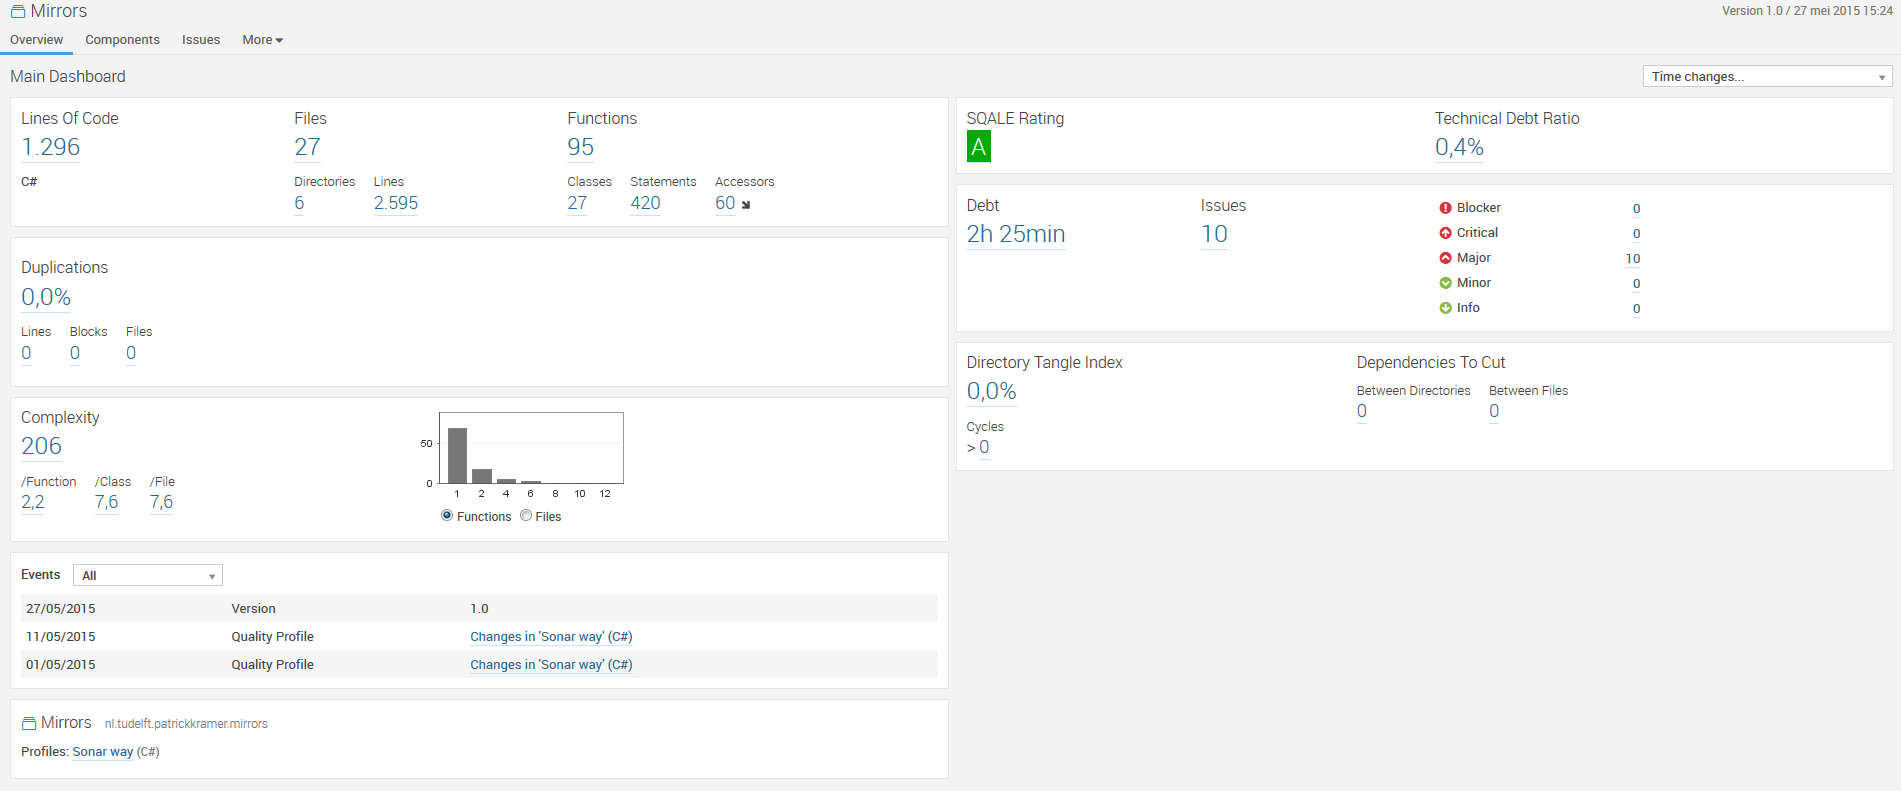
\includegraphics[width=\textwidth]{SonarQube}
			\caption{A SonarQube overview.}
			\label{fig:sonarqube}
		\end{figure}
		
		An issue with SonarQube is that, while it has free options for analyzing
		C\# code, it has none of these free options for analyzing C/C++ code,
		because of the preprocessing that can happen in C or C++ (as explained
		in their blog on \url{http://www.sonarqube.org/ccobjective-c-dark-past-bright-future/}).
		For this reason, it is very hard to analyze the C++ code that we use for the
		OpenCV server.
		
	\section{SIG Evaluation} \label{sec:sigevaluation}
		SIG is an acronym which stands for the Software Improvement Group,
		which is a company that is based in Amsterdam. The company does code
		analysis to evaluate code quality on a scale from one to five stars,
		and it does so according to the ISO/IEC 25010 model. Code score is 
		based on the maintainability of the code.
		
		During the project, there are two opportunities to deliver the code 
		that we have written to SIG. The first opportunity is at the end of 
		May, and the second is halfway through June. The first opportunity 
		is used as a midterm quality feedback session, for us to get feedback 
		about how good the code is written and what can be done better. The 
		second opportunity is then intended to hand in the improved code, 
		and for us to then get feedback on how well the code has been improved. 
		The improvements in the code also have a weight in the final result 
		for the project.
		
	\section{Demo's and playtesting sessions} \label{sec:demos}
		%TODO Write about the demo with the client.
		...

\chapter{Conclusion} \label{cha:conclusion}
In short, the mirror game seems the best solution to the problem. It is a viable project
to create in the given time frame, it is a challenging puzzle game even when playing a 
different version of it (a single-player version) on your own, and it taxes the communication
of both the remote and the local players, as they both have abilities necessary for
achieving the goal, but they cannot achieve it on their own (although this could be relaxed
to make the game more playable). Also, it is still a challenging project, because of the
technical challenge of integrating AR hardware and recognition of markers with the game
world. Additional complexity, such as colored laser beams/targets, beam splitters, beam mergers
etc. could also be implemented to increase the technical challenge of the problem.

The game and networking will be implemented using Unity, with the Vuforia library
handling augmented reality for the local players. The remote players will likely
be using an Oculus Rift and the local players one of the augmented reality devices
describes in the problem analysis that ends up working best in practice.
	% Summarizes the Research Report and provides 
	% an overview and conclusion of the technologies 
	% we're going to use.
	% TODO AR tech elaboration.	

Using this information, we've built a small demo that uses Vuforia. It places
a laser emitter, mirror and wall on three markers that can be moved around. The
mirror reflects the laser realistically based on the angle of incidence.

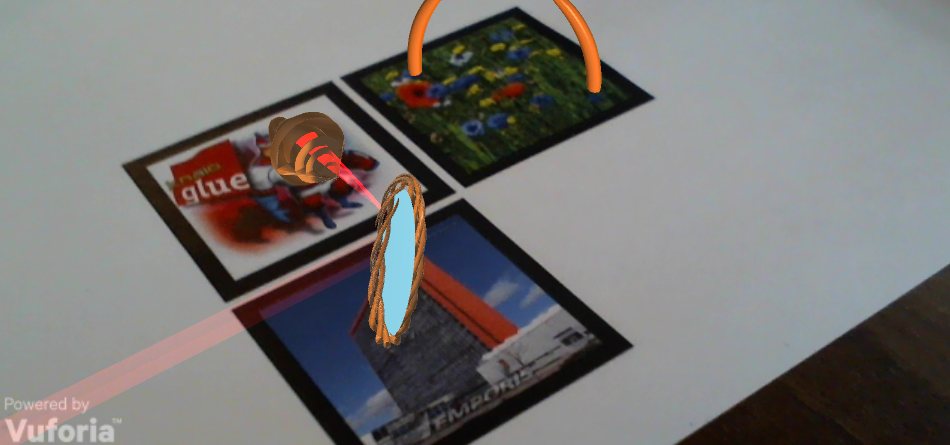
\includegraphics[scale=0.7]{demo.png}

\appendix

\chapter{Research Report} \label{app:researchreport}
\chapter{Problem Formulation} \label{cha:problem}
	% The problem description is taken from BEPSys. It has been shortened 
	% and slightly modified to fit the context of this document.
	While augmented reality research has grown into a mature field over the 
	last years, the aspects of situational awareness and presence of 
	augmented reality (AR) are still quite open research topics. This 
	project is about designing and implementing a collaborative game to 
	explore the different perception of situational awareness, presence and 
	workload in a physical and an AR environment. The game is to be employed 
	as an approximation of collaboratively solving complex problems, as they 
	occur in crime scene investigation when using virtual co-location, i.e. 
	expert remote crime scene investigators to guide local investigators in 
	AR to collaboratively analyse the crime scene. 
	
	It has to be possible to play the game with at least three players: At 
	least two players are present at the same location (physically 
	co-located). At least one player is physically remote but virtually 
	co-located \cite{bepsys}. The game itself should also be unable to be
	completed without either the physically co-located players or the 
	virtually co-located players, however this constraint could be relaxed
	to allow a higher playability of the game (because it would be nice to
	play the game without having to search for a virtually co-located player,
	for example).
	
	%TODO Add our interpretation to avoid ambiguities

\chapter{Problem Analysis} \label{cha:analysis}
	% Includes the challenges surrounding AR and Networking.
	% Also motivates the choices made.
	This chapter provides an analysis of the problem description of problems
	and challenges that may arise during development. It provides an analysis 
	of the problems and possible solutions that can be used in order to 
	solve these problems. 
	
	One of the core challenges of the project is the use of Augmented Reality 
	(AR) technology. An analysis of the available options to implement this 
	functionality is given in section \ref{sec:ar}. Another important challenge
	is improving situational awareness, which is discussed in section 
	\ref{sec:awareness}. The last challenge is the creation of interdependence 
	between players in such a way that requires collaboration from all players.
	This challenge is analyzed in section \ref{sec:interdependence}. 
	
	Lastly, a conclusion based on the analyses of these challenges is given in
	section \ref{sec:analysisconclusion}.
	
	\section{Augmented Reality (AR) Functionality} \label{sec:ar}
		% AR is a core element in the project. As such, we need to compare
		% various AR hardware devices and corresponding ways to implement
		% AR functionality for each device.
		Augmented Reality (AR) is a core aspect of the problem formulation. 
		As such, careful analysis has to be done as to how the AR functionality
		can be best implemented to fully address the context of this project.
		
		We consider two choices for implementing AR functionality: The META One,
		an optical see-through device (\ref{ssec:metaone}), and the Oculus Rift 
		Virtual Reality glasses in conjunction with mounted cameras 
		(\ref{ssec:oculusrift}).
	
		% Hardware devices to consider:
		\subsection{META One} \label{ssec:metaone}
			%   - META One (as indicated by the BEPSys project page)
			%       - Has a limited Field-of-View (around 35 degrees)
			%          - May interfere with the experience of the game.
			%       - Optical see-through glasses means AR works out of the box.
			
			The META One glasses are optical see-through glasses. Optical 
			see-through glasses work by projecting a virtual image on top of the
			world you see, effectively implementing a 3D AR exprience.
			
			Because the META One is an optical see-through device that also 
			features motion tracking, AR can be implemented simply by 
			projecting an image against a black background to the glasses.
			
			A big drawback of the available META One glasses is their 
			Field-of-View, which is 35 degrees. This Field-of-View is way lower
			than the Field-of-View of a person, which may have a negative impact 
			on the game experience.
			
		\subsection{Oculus Rift} \label{ssec:oculusrift}
			%   - Oculus Rift + mounted cameras (http://oculusvr.com/)
			%       - High Field-of-View (100 degrees)
			%       - VR glasses, so need to project the real world using cameras.
			%          - Limited resolution creates blurriness.
			%          - Projection can be done from within Unity
			%          - Potentially requires a lot of calibration
			% 		- Using Oculus Rift means we need to implement AR functionality 
			%         ourselves (as optical see-through often has this built-in).
			%         AR Libraries to consider:
			We've built a camera rig for the Oculus Rift that can be used to
			turn it into an augmented reality device. To detect the markers and
			render objects on them in Unity, there are several libraries
			available. Each of these will be discussed in the next sections.

			Oculus offers an SDK for Unity that makes it easy to integrate a
			game with the Rift. The challenge that we'll be facing during
			development is to properly integrate this SDK with the augmented
			reality libraries. Each of the frameworks try to take control of the
			camera in different ways and it's easy to get conflicts there.
			Getting the Rift see-through functionality working in Unity on its
			own and the augmented reality functionality on its own is not a
			challenge.

			\subsubsection{Vuforia} \label{sssec:vuforia}
				%   - Vuforia (http://vuforia.com/ and http://developer.vuforia.com/)
				%       - Includes integration with Unity
				Vuforia is a framework by Qualcomm that allows you to create
				arbitrary markers, import them into Unity and place objects onto
				them. You can then select a webcam and have it render the camera
				images with 3D objects projected onto the markers. It's very
				easy to use and has built-in support for virtual reality
				solutions like GearVR. The tracking quality is very good and
				stable, even with low quality markers (with few color transitions).

				Unfortunately it currently only works with the 32-bit version of
				Unity. It also lacks support for the Oculus Rift on the desktop,
				which means that we'll have to build that functionality ourselves.

			\subsubsection{Unity AR Toolkit (UART)} \label{sssec:uart}
				%   - Unity AR Toolkit (UART) (https://research.cc.gatech.edu/uart/content/contents/)
				%       - Source code and demos hosted on SourceForge (http://sourceforge.net/projects/uart/)
				%       - Seems to be a research project
				%       - Seems easy to use (comes with examples)
				%       - Built for Unity
				%       - Last change to SVN repo was in 2011.


			\subsubsection{Metaio} \label{sssec:metaio}
				%   - Metaio (http://www.metaio.com/)
				%       - Mainly oriented towards mobile phones, so may not be suitable for this project
	
		%   - ... <Add more as needed>
	
	\section{Situational Awareness} \label{sec:awareness}
		% Improving situational awareness is part of the main goal of the project.
		% We should indicate the steps needed to achieve this, which can be based 
		% on (possibly) a large range of scientific articles.
		This project is about exploring the different perception of situational 
		awareness, presence and workload in a physical and an AR environment 
		(see chapter \ref{cha:problem}). As such, situational awareness plays a 
		key role in this project.
		
	
	\section{Interdependence between players} \label{sec:interdependence}
		% Creating interdependence between players requires them to work together.
		% This can be done in several ways. We need to elaborate on the various ways
		% in which this can be achieved.
		The problem formulation states that the game is to be employed as an 
		approximation of collaboratively solving complex problems. In order to
		motivate players of the game to collaborate, there is a need to create
		a form of interdependence amongst the players. One way to do this is to 
		create an asymmetry between either the information that the players have or
		an asymmetry of abilities, as explained in the following subsection. 
		\subsection{Reasons to co-operate}
			The main reason to co-operate is the asymmetry of abilities between
			the players involved. For example: the physically co-located players
			have the ability to put down mirrors, and the virtually co-located
			players can then rotate the mirrors. Furthermore, information
			asymmetry can also be implemented, for example by allowing only the
			virtually co-located players to see the obstacles. Because of physical
			separation, asymmetry should be focused on physical abilities.
		
	\section{Virtual Co-location} \label{sec:virtualcolocation}
		Establishing virtual co-location is required to allow physically remote players
		to play the game together. As such, both the virtualization of the game world and
		the networking are considered in virtually co-locating physically remote players.
		Unity has multi player support, because of its master server to handle multi player
		games, but the server could be down at times. There are tutorials on the internet
		to create a basic multi player game that uses the master server to handle requests.
		These tutorials can be used to implement our own multilayer support. Alternatively
		we could provide the players with the means to easily get and exchange their IP
		addresses through other means such as mail. 
		Besides the networking we have to look at how we synchronize locations, depending on
		the chosen game we have in order of ascending complexity several options:
		1 Use markers with a known locations, this only works if we have a limited size 
		and reasonably fixed playing area which we can prepare ahead of time. This most 
		likely comes in the form of a set of markers at the edge and middle of the playing 
		field. 
		2 Use mobile markers which synchronize between players automatically, for example
		cards in a card game. This only works if we can trust the play er to keep these markers
		within their screen or if it does not matter if there is no augmentation needed if they
		cannot see a marker. 
		3 Object recognition which tracks the locations of objects in the scene,
		this method only works if there are a number of reasonably stable objects 
		within the player's vision. 
		4 Combining the output of a compass, a gyroscope and trilocations. This is 
		works regardless of what is visible but requires accurate trilocation which works
		can be quite hard to do without building a heavy rig. 
		Of course a combination of several of the above methods is also possible. 

		Then there is the matter of making the players "feel" that they are in the 
		same location. One obvious method might be to put an oculus on the remote player(s) and let 
		them see through the eyes of the local player(s), however this is likely to cause nausea. 
		Of course we can do away with the oculus but that might result in relative pasivism from 
		the remote players as they feel they cannot 
		even control their own view while not being forced to watch what the other player does. 

		We can also let the remote player control one or more avatars within the game world
		and view these through either oculus or screen. This would keep the remote player
		more interested by giving more of a feeling of agency then just viewing through the eyes 
		of the other player at the cost of the feeling of connectivity. But this would require 
		mapping out a large part of the scene in the virtual world. 
		
		Lastly we can also let the remote player view the world from a birds eye perspective 
		this can either be done by mounting a camera above the scene or by rendering it in 
		the virtual world, the second case offers increased player agency resulting in 
		a better attention to the situation at the cost of having the map the scene fully 
		in the virtual world. 
		
		% Allowing phsyically remote players to play the game, we need to establish
		% some idea of virtual co-location. This includes the virtualization of the 
		% game world as well as the networking functionality required to establish
		% the actual connection.
		
	\section{Analysis Conclusions} \label{sec:analysisconclusion}
		\section{Analysis Conclusions} \label{sec:analysisconclusion}
  % Provides the coices we made for the abovementioned problems along with a short
  % motivation based on the above analysis.
  
		% Provides the coices we made for the abovementioned problems along with a short
		% motivation based on the above analysis.

\chapter{Proposed Solutions} \label{cha:solution}
	% A description of the proposed solution, including gameplay elements.
	% The description is taken from the Product Plan. This section also
	% motivates why the proposed solution is a good solution.

\section{Laser mirror game} \label{sec:lasergame}
	The goal of the game is to solve a puzzle by controlling laser beams
	using mirrors in such a way that a predefined target is hit. The game
	can be played by one or more local players and one or more remote players.

	There are cards present for the local players that represent mirror
	bases. These must be placed on the table, which will be the locations
	for the mirrors. The local players will be able to see the mirrors they
	place through the use of AR technology. Each of the local players will
	only be given a few of the mirror bases needed to solve the puzzle, and
	as such solving the puzzle requires cooperation from all local players.

	The remote players can also see the placed mirrors, and can rotate them
	to influence the path of the laser beam(s). Only by cooperation between
	local players (who can only move the mirror bases) and remote players
	(who can only rotate them) it becomes possible to hit the target and as
	such solve the puzzle.

	The game provides various different types of mirrors with different
	properties, allowing for more complex puzzles. One example of such a
	mirror is a colored mirror, and then require the target is hit with the
	right (combination of) colors. Another way to make puzzles more complex
	is requiring that the players combine beams together to create more
	powerful beams. Other optical components like beam splitters can also be introduced.

	The game is designed to stimulate cooperation between the physically
	co-located players and the physically remote player(s). It does so by
	dividing abilities required for solving the puzzles amongst all players
	as follows:

	\begin{itemize}
		\item Physically co-located players each get only a part of the
		      mirror bases required to solve the puzzle, requiring input
		      from all of these players.
		\item If there are multiple virtually co-located players, each of
		      these players can only rotate a subset of the mirrors, and
		      as such input from all virtually co-located players is
		      required for solving the puzzle.
		\item Virtually co-located players have the ability to rotate
		      mirrors while the physically co-located players do not have
		      this ability, requiring input from both physically as well
		      as virtually co-located players.
	\end{itemize}

	Because of this division of abilities, there is an interdependence
	between all players (see section \ref{sec:interdependence}), regardless of
	whether these players are physically co-located or not. This replicates the
	interdependence that exists in the crime scene example as given in the
	problem formulation (see chapter \ref{cha:problem}).

\section{Platformer} \label{sec:platformer}
	The game starts with the avatar of the remote player appearing
	on the table and a goal appearing above the table. The local
  players have a pile of blocks, each of these blocks exists both
  in the virtual and real world.

	Inside the virtual world a number of pre-existing structures and
	obstacles exist making it harder for the remote player to move around.
	The local and remote player must work together in order to get the
	virtual avatar to the goal.

	Team work is heavily encouraged due to the interdependence between the
	players: There is information asymmetry (section \ref{ssec:information})
	because the remote player can see some pre-existing blocks the local
	player cannot see, and the fact that local players can place new blocks
	in the game world provides ability asymmetry (section \ref{ssec:ability}).

\section{FPS Survival game} \label{sec:fpssurvival}
	The goal of the game is to protect a virtual structure from enemies. These
	enemies will come from multiple sides to attack the structure while the
	remote players have to stop them. For doing so, they require the aid of the
	local players, who can place blocks (similar to the platformer game, section
	\ref{sec:platformer}) to block the path of the enemies.

	The local players can block the path of the enemies, but they cannot defeat
	them. The remote players, who view the game from a first-person perspective,
	have to defeat the enemies. Since the perspective of the remote players is
	limited (also partly because of the blocks placed by local players), they
	require information from the local players, who view the scene from above
	and as such have a good view of the entire situation. This creates
	information asymmetry between the players (section \ref{ssec:information}).

	To keep the game challenging, the enemies will grow stronger over time,
	requiring the cooperation between the local and remote players to improve
	as well. Because of the fact that local players can only defeat the enemies,
	and the remote players can block their path, there is a form of ability
	asymmetry between the local and remote players (section \ref{ssec:ability}).

\section{Tower defense} \label{sec:towerdefense}
	The local players start off with a number of towers each
	which have certain strengths and abilities. They must place
	these towers on a table in front of them. What they cannot
	but the remote player can see is what paths a number of
	hostile entities will take in order to attack their base.
	They must therefore cooperate to place the towers on the right
	positions to be able to defeat the enemies before they escape
	by communicating the ideal locations of the
	towers and paths that the hostile entities will take.

	This game idea is relatively simple, and because of the simplicity,
	complexity can easily be added to make the game more engaging. For
	example, towers could be upgradeable, utilizing resources that
	could be gained either by defeating individual enemies or by defeating
	a wave of enemies. These resources could then be used to upgrade
	tower types. As these resources are shared, and they can only be
	used once, players must work together to choose the best upgrade
	available in the given scenario. Enemies should also get procedurally
	stronger because of the increased capabilities of the towers.

	The problem with this idea is that it will very likely create a
	"puppet master" scenario where the remote player takes charge
	of the whole situation and the other players do not get a
	say in what is going to happen. This could be avoided by a
	number of extra abilities. This game shows heavy
	information and ability asymmetry.

\section{Minesweepers}
	This concept is based on the classic game of minesweeper. There's a grid
	where some of the squares have mines under them. Players each start at a
	random position and have to place flags on locations of mines while avoiding
	mines. The remote player is the only one who can see the numbers around
	squares, so he has to give instructions to the players on the field.

	The difference compared to the classic version of the game is that it's all
	physical. Local players walk around on the field, where they have to take
	careful steps to avoid triggering a mine. This turns the game into some sort
	of Twister variant where people can use special moves to quickly traverse
	the field and find all the mines. Local players co-operate by dividing the
	field into sections that they'll clear in parallel.

	The problem with this concept is the inherent *puppet master* phenomenon.
	Communication between the remote player and local players is very one-sided.
	Local players just receive commands where to step and where to plant flags
	and don't really have any input into the game themselves. Even if that
	problem was solved, the lack of cooperation aspects between local players
	would also be a big problem. Local players don't really have any reason to
	interact with each other. One way to solve that problem would be to require
	multiple players to place a flag.

	There are also some technical challenges with this concept. It requires that
	local players always know their exact position on a large field that they're
	inside of, which would require a lot of markers. Next, the position of their
	legs would have to be determined somehow to ensure that they're not stepping
	on a mine. Finally, a space large enough for a field would likely have to be
	found outside and sunlight doesn't play well with augmented reality devices.

\section{The chosen idea} \label{sec:chosenidea}
	The idea that is chosen is the mirror game idea. The reason for this
	decision is that it is a relatively simple idea, it can create hard
	to solve puzzles, and extra complexity can easily be added. It also
	prevents a "puppet master" scenario by giving both types of players
	about half of the abilities required for solving the game.

\chapter{Conclusion} \label{cha:conclusion}
In short, the mirror game seems the best solution to the problem. It is a viable project
to create in the given time frame, it is a challenging puzzle game even when playing a 
different version of it (a single-player version) on your own, and it taxes the communication
of both the remote and the local players, as they both have abilities necessary for
achieving the goal, but they cannot achieve it on their own (although this could be relaxed
to make the game more playable). Also, it is still a challenging project, because of the
technical challenge of integrating AR hardware and recognition of markers with the game
world. Additional complexity, such as colored laser beams/targets, beam splitters, beam mergers
etc. could also be implemented to increase the technical challenge of the problem.

The game and networking will be implemented using Unity, with the Vuforia library
handling augmented reality for the local players. The remote players will likely
be using an Oculus Rift and the local players one of the augmented reality devices
describes in the problem analysis that ends up working best in practice.
	% Summarizes the Research Report and provides 
	% an overview and conclusion of the technologies 
	% we're going to use.
	% TODO AR tech elaboration.	

Using this information, we've built a small demo that uses Vuforia. It places
a laser emitter, mirror and wall on three markers that can be moved around. The
mirror reflects the laser realistically based on the angle of incidence.

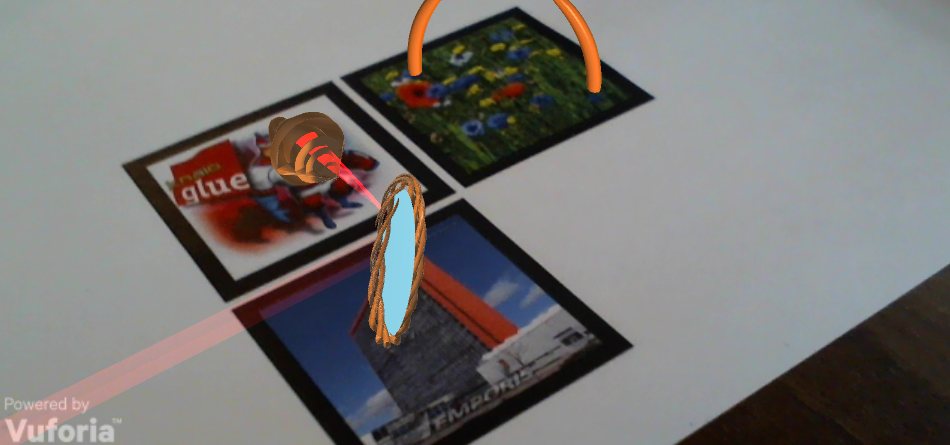
\includegraphics[scale=0.7]{demo.png}

\chapter{Product plan} \label{app:productplan}
\section{Concept}
This section covers the concept idea of the gameplay, and the accompanying
requirements.

\subsection{Gameplay}
The goal of the game is to solve a puzzle by controlling laser beams using mirrors
in such a way that a predefined target is hit. The game can be played by 
one or more local players and one or more remote players.

There are cards present for the local players that represent mirror bases. These 
must be placed on the table, which will be the locations for the mirrors. The local
players will be able to see the mirrors they place through the use of AR technology.
Each of the local players will only be given a few of the mirror bases needed to solve
the puzzle, and as such solving the puzzle requires cooperation from all local players.

The remote players can also see the placed mirrors, and can rotate them to influence 
the path of the laser beam(s). The remote players is also the only one who can see the
obstacles that are predefined for that particular puzzle. Only by cooperation between 
local players (who can only move the mirror bases) and remote players (who can only 
rotate them) it becomes possible to hit the target and as such solve the puzzle.

The game provides various different types of mirrors with different properties, 
allowing for more complex puzzles. One example of such a mirror is a colored mirror, 
and then require the target is hit with the right (combination of) colors. Another 
way to make puzzles more complex is requiring that the players combine beams together
to create more powerful beams. Other optical components like beam splitters can
also be introduced.

\subsection{Requirements}

\paragraph{Must haves}
\begin{itemize}
	\item A light source, a target and zero or more blocks must be visible when the game starts.
	\item A light source must emit a light beam in a predefined direction.
	\item A light beam must reflect against a mirror when it hits one.
	\item A light beam must stop when it hits a block
	\item A local player must be able to see mirrors over the cards using AR technology.
	\item A local player must be able to move the mirrors by moving the cards.
	\item A remote player must be able to see the mirrors in the same positions and 
		  orientations as the local players.
	\item All players must be able to see the light beam, the light source, the target and the blocks.
	\item A remote player must be able to rotate the mirrors.
\end{itemize}

\paragraph{Should haves}
\begin{itemize}
	\item There should be elevations of mirrors, to allow light of a lower elevation to hit the target on a higher elevation, or the other way around
	\item The light beams should be colored (after a certain level), and only light beams of a certain color can suffice in hitting the target.
	\item There should be combiners (think AND- or OR-gates) that combine light and cause it to travel to the target.
	\item There should be color combiners, to allow for a broader variety of color-specific targets.
\end{itemize}

\paragraph{Could haves}
\begin{itemize}
	\item The game could have an infinite amount of levels.
	\item The game could have random level generation according to maximum difficulty settings.
	\item The game could give hints if the players are stuck.
\end{itemize}

\paragraph{Won't haves}
\begin{itemize}
	\item The game won't be playable with only remote players.
	\item The game won't be playable with only local players.
	\item The game won't be playable on Android or iOS devices.
\end{itemize}

\section{Approach}

This section covers development details that aren't directly related to the
gameplay itself, such as software engineering practices and guidelines about
client meetings.

\subsection{Technical details}

technische details, zoals gebruik van ar toolkit en oculus rift + camera's

\subsection{Software engineering}

test coverage, scrum, UML, testen met gebruikers

\subsection{Guidelines}

Here is a list of rules that help prevent problems during development.

{\color{red} NOTE: These are just ideas right now}

\begin{itemize}
	\item Send a progress report to the client at least once a week
	\item Meet with the client and coach once every 2 weeks to show a working demo
\end{itemize}
\section{Planning}

The first two weeks represent the research phase. In this phase we will find a suitable augmented reality (AR) library for Unity and prepare an Oculus Rift for AR use with cameras. We'll also design an architecture for the game that covers the marker detection, networking and gameplay mechanics. All of this information will be described in the research report handed in on May 1st. Main development commences after this phase and is organized in weekly sprints. The table below describes the goals per sprint, which will serve as a helpful reference to stay on schedule during development.

The first SIG submission is due May 26th. By then, we should already have a semi-functional product. The basic functionality (AR functionality, basic gameplay mechanics, etc.) should be in this version of our product. All the relevant graphics assets should also be done.

The second SIG submission is due June 6th. By then, most of the functionality should be implemented (this includes advanced gameplay mechanics, hitting multiple targets, mirror elevations, etc). Also, all the bad parts of the code structure/architecture from the first version should be resolved.

The project should be done by June 26th, the Friday of week 4.10. This includes not only the project but also a final report of 40 to 50 pages. This means that the report should be worked on continuously.
 
\begin{tabular}{|l|c|r|}
	\hline
	Weeks      & Deadline  & Goal \\ \hline
	4.1 + 4.2  & May 1st   & Research report described above \\ \hline
	4.3        & May 8th   & AR integration + lasers \\ \hline
	4.4        & May 15th  & Basic gameplay start + start report \\ \hline
	4.5        & May 22nd  & Finalize first SIG version \\ \hline
	4.6        & May 29th  & Start advanced gameplay \\ \hline
	4.7 + 4.8  & June 12th & ??? \\ \hline
	4.9 + 4.10 & June 26th & ??? \\ \hline
\end{tabular}

\subsection{Holidays + businessdays on which EWI is closed}

\begin{tabular}{ll}
	Koningsdag               & 27-04-2015 \\
	Dodenherdenking          & 04-05-2015 \\
	Bevrijdingsdag           & 05-05-2015 \\
	Hemelvaartsdag           & 14-05-2015 \\
	De dag na Hemelvaartsdag & 15-05-2015 \\
	2e Pinksterdag           & 25-05-2015
\end{tabular}


\pagebreak
\addcontentsline{toc}{chapter}{Bibliography}
\bibliography{Bibliography}

\end{document}
